% -*- latex -*-
% FILE: "/home/evmik/jobs/wm/2012_spring_Analog_Electronics_252/final_exam/questions/noninverting_amplifier_with_opamp.tex"
% LAST MODIFICATION: "Tue, 01 May 2012 01:08:13 -0400 (evmik)"
% (C) 2011 by Eugeniy Mikhailov, <evgmik@gmail.com>
% $Id:$

\question{}
	Consider the non inverting amplifier shown below \\
	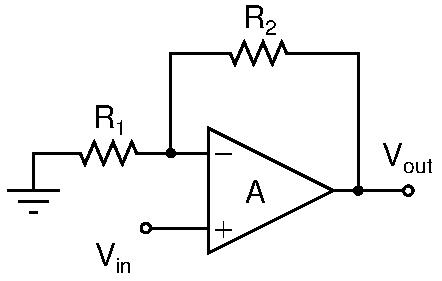
\includegraphics[height=1in]{./schematics/noninv_ampl}\\
	\begin{parts}
		\part[10]
		Find the expression for the output voltage in terms of $V_{in}$,
		$R_1$, $R_2$, and $A$. Do not assume that $A$ is infinite.
		\vskip 2.5in
		$V_{out}=$
		\part
		If the gain bandwidth product $A(f) \times f = 10$~MHz.
		$R_2/R_1=10$.
		\begin{subparts}
			\subpart[5]
			What is the gain of the system at 10~Hz
			\vskip 0.5in
			$G(10~Hz)=$
			\subpart[5]
			What is the gain of the system at 10~MHz
			\vskip 0.5in
			$G(10~MHz)=$
		\end{subparts}

		\part[5]
		Consider the practical limitations now.
		If  $R_2/R_1=99$, $V_{in}=0.01$~V, and $A=\infty$, 
		but maximum output current of the
		Op-amp is 2~mA. What is the minimal possible load resistor which you
		can hook to the output without overloading the Op-amp?
		Assume that $R_2 \gg R_L$.

		\vskip 0.5in
		$R_{L_{min}}=$
		\bonuspart[5]
		What is the output impedance of this amplifier at low
		frequencies?  
		{\bf Why} do you think so?
		Assume $A=\infty$.
		\vskip 0.4in
		$Z_{out}=$
	\end{parts}
	\pagebreak

